\subsection{Training ViT}
Results visible in next pages were obtained using ViT model trained with following hyperparameters, visible on \prettyref{lst:vit-hyperparameters}.

\newenvironment{longlistingI}{\captionsetup{type=listing, width=0.8\textwidth}}{}
\begin{longlistingI}
    \pythoncode{listings/vit_hyperparameters.py}
    \caption{ViT model initialization}
    \label{lst:vit-hyperparameters}
\end{longlistingI}
\vspace{12pt}

For the training phase, 90,000 samples were generated, comprising 10,000 samples for different number of elements ranging from 0 to 9. 
90\% of the samples were utilized in the training step, while the remaining 10\% were allocated for the validation. 
The Adam optimizer was employed with a learning rate of 0.0001, and Binary Cross Entropy loss was used because multi-label classification reduces to multiple binary classification problems.

The model was trained for 10 epochs, with a batch size of 128 and loss through epochs can be seen on \prettyref{fig:vit-loss}. Training loss was averaged over all mini batches in epoch, which is why it is generally larger than validation loss, which was calculated after the epoch. 

After training, the ROC (Receiver Operating Characteristics) curve over 5000 random samples was calculated to assess the model's performance. 
The ROC curve is a plot of $recall$ ($sensitivity$) against \(1-specificity\) \cite{rocCurve}. 
Recall, also known as the TPR (True Positive Rate) says what part of all positive instances was classified correctly and is defined as \(\frac{\text{TP}}{\text{TP} + \text{FN}}\) (look \prettyref{tab:classification_matrix} for abbreviations).
$1-specificity$, or FPR (False Positive Rate) is defined as \(1 - \frac{\text{TN}}{\text{TN} + \text{FP}}\) and says how many positive instances were classified incorrectly.
When the threshold for positive classification, e.g., 0.5, is lowered, the number of positive classifications increases, resulting in an increase of both TPR and FPR. 
However, lowering the threshold will lead to an increase in false positives, possibly greater than true positives, causing the \(\frac{\text{TPR}}{\text{FPR}}\) ratio to decrease.

In general, better classifiers should have a greater area under the ROC curve, known as AUC (Area Under the Curve). 
The ROC curves and AUCs of different classes, calculated for the trained model are visible in \prettyref{fig:roc-auc}.

\begin{table}[htbp!]
  \centering
  \begin{tabular}{|c|c|c|}
    \hline
    & \textbf{Real Positive} & \textbf{Real Negative} \\
    \hline
    \textbf{Predicted Positive} & True Positive (TP) & False Positive (FP) \\
    \hline
    \textbf{Predicted Negative} & False Negative (FN) & True Negative (TN) \\
    \hline
  \end{tabular}
  \caption{Classification matrix}
  \label{tab:classification_matrix}
\end{table}

\begin{figure}[H]
  \centering
  \includesvg[width=0.8\textwidth]{img/vit_loss.svg}
  \caption{Loss in each training epoch}
  \label{fig:vit-loss}
\end{figure}


\begin{figure}[htbp!]
  \centering
  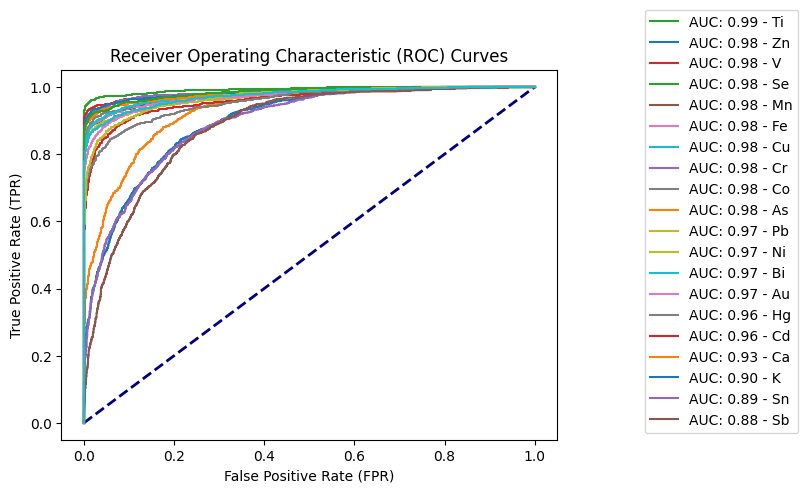
\includegraphics[width=1\textwidth]{img/roc_auc.png}
  \caption{ROC and AUC of each trained element}
  \label{fig:roc-auc}
\end{figure}

ROC of a few spectral lines, namely Ca, K, Sn, and Sb, seems to differ significantly from the rest. 
The energies of their spectral lines are as follows: 3.692, 3.314, 3.444, and 3.604 [keV]. 
As one can see, these values are quite close to each other, and the elements do not have any other lines defined in the code that could help differentiate between elements.
In that case model could be improved by using more accurate theoretical element spectra. 

Besides ROC, a few metrics were evaluated for different number of elements in spectra, namely: accuracy, precision, recall and f1 score. 
Precision is evaluated as $\frac{TP}{FP+TP}$, representing the proportion of instances classified as positive that were correctly identified.
f1 score is popular metric that unifies precision and recall under one metric as a harmonic mean -  $2\times\frac{precision \times recall}{precision + recall}$.
The evaluation was conducted on 1000 random samples within each category and is visible on \prettyref{fig:vit-scores}.

\begin{figure}[htbp!]
  \centering
  \includesvg[width=0.8\textwidth]{img/vit_equal_classes_scores.svg}
  \caption{Loss in each training epoch}
  \label{fig:vit-scores}
\end{figure}
